Workflow is loosely defined here. Inevitably, refinements will be made as issues are discovered and resolved. The acquisition process, from capture to ingest, can be imagined as a pipeline starting from the physical original and ending with an archival Submission Information Package (SIP). Stages in this pipeline include: page scanning, OCR text extraction, OCR cleanup, baseline TEI encoding and Submission Information Packaging (SIP).
\begin{figure}[H]
  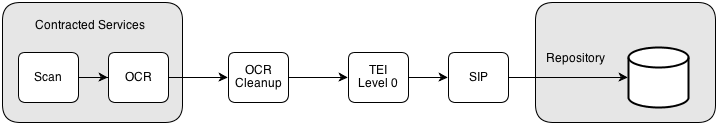
\includegraphics[width=0.8\textwidth]{sip-pipeline.png}
  \caption{from capture to ingest}
\end{figure}
%This chain of functions can be represented as $SIP ::= TEI(text(scan(page)))$
While each stage will require human intervention and oversight, the OCR correction stage is expected to incur the most significant outlay of human resources. 
\subsection{Contracted Services}
The raw scans and text will be provided by Hill Memorial Library as a contracted service. Details of this process will be handled by library staff, and the end product will be delivered to the project team for further pre-ingest processing. As noted elsewhere, Hill will retain a copy of this corpus in perpetuity.

\subsection{Data Structure}
\subsubsection{Image + Text}
The atomic elements of the repository are garden variety TIFF images and lightly-encoded\cite{tei_sig_on_libraries_best_2011} TEI text files. The most basic use-case for repository records is that of an end-user browsing one of the issues of \bwj{}, for example. In this scenario, the user expects to view the page image, but also to have the ability to search the text for keywords, for example, all occurrences of the word \emph{election} occurring in the current, say, June 1844 issue. A list of search results comes back, the user chooses one to follow.

The collection is comprised of a subset of all the issues of four periodicals. Each issue contains pages; each page contains text, possibly a heterogeneous concatenation of text from two or more adjacent pieces, advertisements, and graphics. This is a complex, but neatly hierarchical, structure that should be represented in a suitable data structure. 

\subsubsection{METS Records}
METS is an XML format for describing the structure of archival digital objects. METS records are used to describe books, for example, where a single METS record represents the book, and nested within this record is a METS record for each page. Each of these page records contains, at a minimum, a reference to the TIFF image of the page and the TEI markup of the text. In addition to describing structure, METS is a container format for other metadata formats. Commonly including in a mets:mdwrap element are RDF elements for semantic mappings, MODS records for bibliographic and library catalog information, EAD finding aids, and so on. It enjoys widespread use and the endorsement of leading archival institutions, including the Library of Congress. 



\subsection{TEI, Level 1}
TEI SIG's Best Practices of TEI in Libraries enumerates five levels of TEI encoding that describe increasingly complex markup. The baseline text for each page will have the characteristics of this Level 1 TEI and will serve as the base upon which enhanced readings are built.
\begin{quote}
\begin{singlespace}
The text is subordinate to the page image, and is not intended to stand alone as an electronic text (without page images). Level 1 texts are not intended to be adequate for textual analysis; they are more likely to be suited to the goals of a preservation unit or mass digitization initiative. Though their encoding is minimal, Level 1 texts are fully valid XML texts. In addition to taking advantage of the TEI header, these texts, while lightly encoded, can be easily combined with more richly encoded texts (that also follow these guidelines) for searching. Further encoding based on document structures or content analysis can be added to a Level 1 text at any time.
Level 1 is most suitable for projects with the following characteristics
\begin{itemize}
    \item{a large volume of material is to be made available online quickly}
    \item{a digital image of each page is desired}
    \item{no manual intervention will be performed in the text creation process}
    \item{the material is of interest to a large community of users who wish to read texts that allow keyword searching}
    \item{sophisticated search and display capabilities based on the structure of the text are not necessary}
    \item{extensibility is desired; that is, one desires to keep open the option for a higher level of encoding to be added at a later date}
\end{itemize}
\cite{tei_sig_on_libraries_best_2011}
\end{singlespace}
\end{quote}
\subsection{OCR Cleanup and TEI}
Cleaning dirty OCR is an intensely human process. Each word in each page must be compared to the original for fidelity; errors will be corrected in standard text-editing software. Dual monitors will be necessary for the staff performing this work. In addition, spell-checking utilities will identify gross errors introduced by the OCR process. While we will aim for perfection, errors will remain. The repository should plan for these future text updates and determine utilities for propogating revisions to derivative versions.
The process of manually correcting OCR text is a prerequisite for the intermediate TEI levels three and four. In the scope of the initial project phase, described here, it is likely that TEI levels above three will be used only for a few proof of concept and highlight cases. Level 2 does not require corrected text and still treats the text as subordinate to the page image while making some additional structural markup. Level three TEI is most fitting at this stage, and the TEI SIG describes it as follows:
\begin{quote}
\begin{singlespace}
Encoding at this level provides the foundation for upgrading to higher levels of encoding. Level 3 generally requires some human editing, but the features to be encoded are determined by the logical structure and appearance of the text and not specialized content analysis.

Level 3 texts identify front and back matter, textual divisions, and all paragraph breaks. Floating texts, or sub-texts like a poem or letter embedded in the greater text, are supported in this level. The finer granularity of encoding these features, as well as figures, notes, and all changes of typography, allows a range of options for display, delivery, and searching. For example, one has the option of identifying, and therefore specifying, the display characteristics of different typographic styles, and regularizing the display and placement of note text.

Level 3 texts can stand alone as text without page images, and therefore can be uploaded, downloaded, and delivered quickly, and require less storage space than digital collections with page images. However, the simple level of structural analysis and absence of specialized content analysis reflected in Level 3 encoding may make it desirable for some, depending on project priorities, to include page images in order to provide users with a fuller set of resources.
\cite{tei_sig_on_libraries_best_2011}
\end{singlespace}
\end{quote}
\subsection{Conclusion}
In a recent CLIR report, warns against insularity in planning Digital Humanities projects and validates this project's aims towards linked data.
\begin{quote}The silo-like nature of current centers is creating untethered digital production that is detrimental to the needs of humanities scholarship. Today’s centers favor individual projects that address specialized research interests. These projects are rarely integrated into larger digital resources that would make them more widely known and available for the research community. As a result, they receive little exposure outside their center and are at greater risk of being orphaned over time.\cite{zorich}
\end{quote}
Given raw images and dirty OCR as a starting point, core project goals may be achieved by identifying a suitable Trustworthy Digital Repository, by coercing the text to TEI Level 3, and by binding page image + text in a suitable format such that each issue of each magazine is available to modern readers much as it was to contemporary readers. Selection of and strict adherence to appropriate standards will ensure that the repository is sustainable for the long-term, that it can serve as a fertile base for deeper investigation, and that it may become part or an increasing community of repositories that have opened their data to use and reuse by others. 




%\begin{description}
%  \item[periodical]{physical original magazine}
%  \item[page]{leaf of a periodical}
%  \item[scan]{digitization of leaf to TIFF}
%  \item[TIFF]{image of leaf}
%  \item[OCR]{process by which text is extracted from TIFF}
%  \item[raw text]{output of OCR}
%  \item[OCR correction]{manual process by which machine interpretation errors are corrected by humans}
%  \item[TEI-1]{baseline format of text for archival storage}
%  \item[SIP]{METS-encoded record of a single periodical issue containing TIFF + TEI of each leaf contained in the original}
%\end{description}

